\documentclass [a4 paper, 11pt, titlepage] {article}

\usepackage{nicematrix}
\usepackage{graphicx}
\usepackage{IEEEtrantools}
\usepackage{multirow}

\addtolength{\hoffset}{-2cm}
\addtolength{\textwidth}{4cm}

\begin{document}
	\title{EE568 Project 4}
	\author{Baris Kuseyri}
	\date{\today}
	\maketitle
	
	\pagenumbering{arabic}
	\tableofcontents
	\newpage
	
	\section{Introduction}

	DW stator topologies are the major stator type used in PMSMs. This is due to their near sinusoidal MMF which yields a high main harmonic winding factor and low torque ripple. It was not until very recently that it was shown that the right choice of slot and pole combination for a FSCW stator could yield a high main harmonic winding factor which is essential to having a high average torque \cite{farshadnia_advanced_2018}









	\subsection{Aims \& Objectives}
	This paper designs an electric motor (EM) to be used as a part of an hybrid electric propulsion system for Cessna 172 Skyhawk. Definition of the hybrid electric propulsion system and the corresponding EM requirements, e.g. rated power, dimensional limitations etc., are outlined in the project proposal. Several EMs with different slot/pole combinations are designed, complying the described requirements. A comparative analysis is performed on these designs, focusing on torque density and cogging torque aspects. One design is chosen, and further alterations are applied to enhance the EM performance. Additionally, this paper proposes a novel winding topology to reduce the cogging torque.


	\section{Literature Review}
	The term FSCW is used to indicate that EM has a non-integral number of slots-per-pole-per-phase $q$,
	\begin{IEEEeqnarray*}{rCl}
		q = \frac{Q}{2pm}
	\end{IEEEeqnarray*}
	where, $Q$ is number of slots, $2p$ is number of poles and $m$ is number of phase.
	
	FSCW topologies are reported to exhibit higher power density. CW comprises of shorter end-windings, resulting with a lower copper loss due to end-windings, compared to DW. FSCW topologies display higher self-inductance, leading to a wider field-weakening region \cite{farshadnia_advanced_2018}.
	The aspect of fault-tolerant in an EM is proportional to several characteristics.
	
	First of all, magnetic coupling between phases, which implies a high mutual inductance, diminishes the fault-tolerancy of an EM. Therefore, phases which are magnetically seperated is desired to achieve a higher fault-tolerancy rating \cite{bianchi_use_2006}. In SPM machines, single-layer winding demonstrates higher self-inductances and lower mutual inductances compared to its double-layer counterparts. A high self-inductance limits the amplitude of short-circuit current, a significant property for fault-tolerancy \cite{el-refaie_fractional-slot_2010} \cite{ishak_comparison_2006}. 
	
	
	Secondly, it is desired to have phases which are physically seperated to achieve fault-tolerancy\cite{bianchi_use_2006}. Lastly, 
	
	
	Mutual coupling between phasesTo achieve a greater fault-tolerant EM
	
	
	Fractional-Slot Concentrated-Winding (FSCW) topology has become of great interest, since it provides a vast amount of choices for the electric motor (EM). 
	
	analytical modelling of the stator MMF and machine equivalent airgap function are essential to correct calculation of the stator magnetic field and inductances, and subsequently torque and torque ripple. analytical formulae for the stator MMF. \cite{farshadnia_advanced_2018}.
	
	\subsection{Torque Density}
	
	\subsection{Torque Ripple}
	3 torque components are present in FSCW PMSM. These are: alignment torque, reluctance torque and cogging torque.
	\begin{IEEEeqnarray*}{rCl}
		T_{em}(t)=T_{align}(t)+T_{rel}(t)+T_{cog}(t)
	\end{IEEEeqnarray*}
	
	Torque generated as a result of the interaction between stator and rotor MMF is alignment torque. $p/2$th harmonic of PM flux linkage, corresponding to fundamental component, contributes to the average alignment torque. Remaining harmonic components provides for the alignment torque ripple \cite{farshadnia_advanced_2018}.
	Torque generated as a result of the stator field aligning the rotor as the reluctance of the magnetic circuit is minimum. Reluctance varies according to the rotor position, while an IPM machine is magnetically salient. This saliency forms as the PM permeability is approximately equals to that of air; thus, contributing to the air-gap length. Similar to alignment torque, $p/2$th harmonic of self and mutual inductance, corresponding to fundamental component, contributes to the average alignment torque. Remaining harmonic components provides for the reluctance torque ripple \cite{farshadnia_advanced_2018}.
	
		
	Cogging torque is one of the torque elements contributing to the torque ripple in the PMSM. The amount of stator teeth aligned with poles in the rotor at a given instance. For the corresponding magnetic circuit, permeance is highest when a rotor pole and a stator tooth are aligned. The system is stable at this point, and the corresponding cogging torque is zero. This results with a force that tries to keep the pole steady; hence, emerging a torque counter to the rotor rotation. This is called 'cogging torque'. More of such alignments result with more cogging torque. 
	The most acknowledged indicator for the cogging torque in a PMSM is the value of least common multiple (LCM) between the number of slots $Q$ and number of poles $2p$. Zhu and Howe (2000) introduce a factor $C_T=\frac{2pQ}{LCM(Q,2p)}$, to assess the cogging torque in a given PMSM. They profess that this factor $C_T$ is directly proportional to the amplitude of the cogging torque \cite{zhu_influence_2000}. Zhu (2011) claims the same as Zhu and Howe (2000), stating that higher LCM and lower GCM between number of slots $Q$ and number of poles $2p$ lead to lower cogging torque. In addition to this, it is argued that machines with a slot/pole combination of $2p=Q\pm2$ exhibit very low cogging torque, while machines with a slot/pole combination of $2p=Q\pm1$ exhibit the lowest cogging torque, with a downside of having unbalanced magnetic force \cite{masmoudi_fractional_2011}. Zhu, Wu and Jamil (2014) inspect machines with slot/pole combinations of $2p=Q\pm2$, $2p=Q\pm1$, $Q/2p=12/8$ and one integer-slot machine $Q/2p=12/4$, assessing the machines in terms of cogging torque, leading to a similar result \cite{zhu_influence_2014}. Jahns and Soong (1996) examine cogging torque in different machines and provide various methods to reduce the cogging torque \cite{jahns_pulsating_1996}. They state that skewing is one of the most popular and most effective way to reduce the cogging torque, if not, eliminate completely. Azar, Zhu and Ombach (2012) utilize skewing method in their work, to reduce the cogging torque. They report that skewing the PMSM by one actual cogging torque period can eliminate the cogging torque and reduce the torque ripple significantly \cite{azar_influence_2012}. Jahns and Soong also mention about winding distribution, increasing number of phases and air-gap winding and their effect on reducing cogging torque when carefully employed \cite{jahns_pulsating_1996}. Additionally, they report the effect of magnet arc width and positioning and its effect on cogging torque \cite{jahns_pulsating_1996}. Work of Ahsanullah, Dutta and Rahman (2013) and Wang, Wang and Jung (2013) show how magnet arc width may reduce the resulting cogging torque \cite{wang_cogging_2013} \cite{ahsanullah_design_2013}. Jahns and Soong (1996) also report the utilization of dummy slots and dummy teeth and how it may result with the reduction of cogging torque \cite{jahns_pulsating_1996}. Zhu and Howe (2000) work on this method, naming not as dummy, but auxiliary, and approve this method for reducing the cogging torque. Bianchi and Bolognani (2002) reports a similar work to Jahns and Soong (1996), reporting similar methods and similar results, with an additional method of PM shifting. Wu and Zhu (2015) reports the effect of tooth tip width on cogging torque and torque ripple in FSCW SPM, and the trade-off between the two torque components in such machine \cite{wu_design_2015}. Finally, Farshadnia (2018) reports similar cogging torque characteristics as Zhu and Howe (2000), reporting in his work about how higher LCM between number of slots $Q$ and number of poles $2p$ indicates lower cogging torque.


	
	FSCW stator topologies are characterized by their slots per pole per phase ratio, denoted $S_{pp}$\cite{farshadnia_advanced_2018}. 
	
	
	
	
	
	
	\section{Analytical Calculation \& Sizing}
	As mentioned in the proposal the machine rating are,
	\begin{table}[h]
		\begin{center}
			\begin{tabular}{c|c|c}
				Power [kW] &  Speed [rad/s] &  Torque [N$\cdot$m]\\
				\hline
				$46.9790$ & $282.7433$ & $166.1542$
			\end{tabular}
		\end{center}
		\caption{Lycoming Operator's Manual IO-360-L2A Operating Conditions}
		\label{fig:EMoperations}
	\end{table}
	

	
	\subsection{Magnetic Loading \& Electrical Loading}
	Permitted RMS values for linear current densities $\bar{A}$, current densities $J$ and peak air-gap flux densities for PMSMs with single-layer field winding, and the corresponding tangential stress $\sigma_{Ftan}$ are reported as follows:
	\begin{table}[h]
		\begin{center}
			\begin{tabular}{c|c|c||c}
				$\bar{A}$ $[kA/m]$ & $\hat{B}_g$ $[T]$ & $J$ $[A/mm^2]$ & $\sigma_{Ftan}$ $[Pa]$ \\
				\hline
				35-65 &  0.85-1.05 & 2-4 & 21000-48000\\
				50 &  0.95 &  & 33876\\
			\end{tabular}
		\end{center}
		\caption{PMSMs with Single-Layer Field Winding }
		\label{fig:EMoperations}
	\end{table}
	Here, $\sigma_{Ftan}$ is calculated by
	\begin{equation}
		\sigma_{Ftan}=\frac{\hat{A}\hat{B}_g}{2}=\frac{\bar{A}\hat{B}_g}{\sqrt{2}}
	\end{equation}
	where, ($\hat{\cdot}$) is for peak value and ($\bar{\cdot}$) is for RMS value of the parameter.
	Therefore, suitable magnetic and electric loading are chosen as
	
	\subsection{Specific Machine Constant}
	\begin{IEEEeqnarray*}{rCl}
		C &=& \frac{\pi^2}{\sqrt{2}}k_w\bar{A}\hat{B}_g=\frac{\pi^2}{2}k_w\hat{A}\hat{B}_g \\
		&=& \frac{\pi^2}{\sqrt{2}}k_w\cdot50\cdot0.95 \\
		&=& 331496.1\cdot k_w [W/m^3]
	\end{IEEEeqnarray*}
	where, $k_w$ is the winding factor.
	
	
	\subsection{Rough Dimensions}
	
	
	\paragraph{Rotor Volume $V_r$} in PMSMs can be calculated in a similar manner with asynchronous machines
	\begin{IEEEeqnarray*}{rCl}
		T &=& \sigma_{Ftan}r_r(2\pi r_rl') \\
		&=& \sigma_{Ftan}V_r \\		
	\end{IEEEeqnarray*}
	\begin{IEEEeqnarray*}{rCl}
		V_r &=& \pi\frac{D^2_r}{2}l'=\frac{T}{2\sigma_{Ftan}} \\
		&=& \frac{166.1542}{2\cdot33876} = 0.0025 [m^3]
	\end{IEEEeqnarray*}

	\paragraph{Air-gap Clearance} in PMSMs can be calculated in a similar manner with asynchronous machines
	\begin{IEEEeqnarray*}{rCl}
		\delta_g &=& \frac{0.18+0.006P^{0.4}}{1000} [m]=\frac{0.18+0.006\cdot46979^{0.4}}{1000} [m] \\
		&=& 6.235195394489506e-04[m] \\
		&\approx& 0.624 [mm]
	\end{IEEEeqnarray*}
	
	\paragraph{Equivalent Machine Length to Air-gap Diameter $\chi=\frac{l'}{D_g}$} in synchronous machines with pole-pair number more than 1, i.e. $p>1$, this ratio is calculated as
	\begin{IEEEeqnarray*}{rCl}
		\chi &=& \frac{l'}{D_g}\approx\frac{\pi}{4p}\sqrt{p} \\
	\end{IEEEeqnarray*}
	where, the $p$ stands for number of pole pairs in the machine. $\chi$ ratio for different number of pole-pairs $p$ can be seen in Fig. \ref{fig:chiRatio}.
	\begin{figure}[h]
		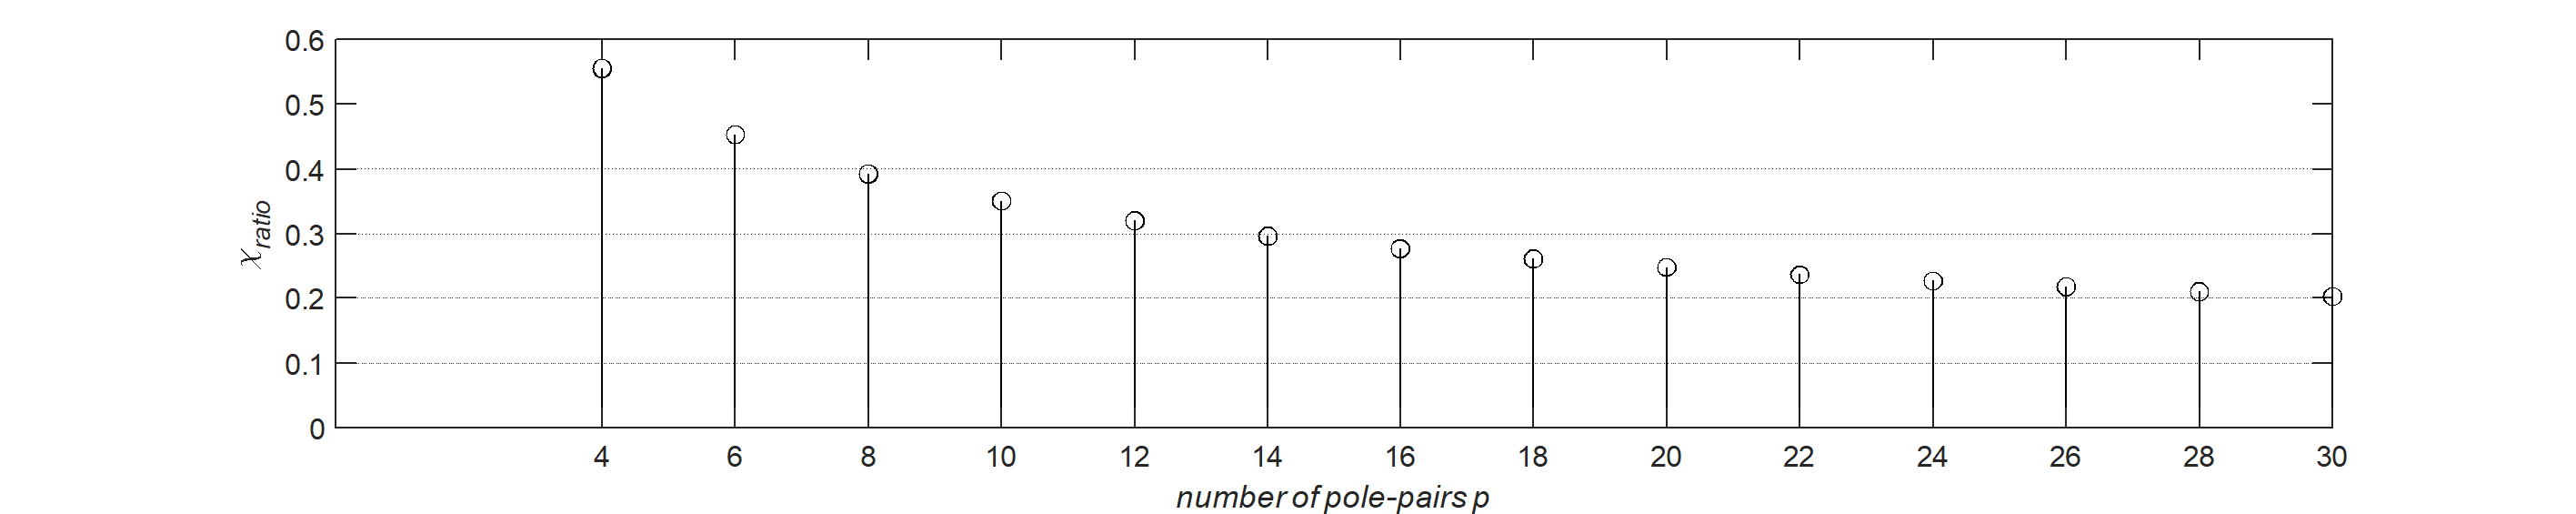
\includegraphics[width=\textwidth]{chiRatio.png}
		\caption{$\chi$ ratio for different number of pole-pairs $p$}
		\label{fig:chiRatio}
	\end{figure}

	
	\begin{table}[h]
		\begin{center}
			\begin{tabular}{c|c}
				 &  \\
				\hline
				airgap clearance & 0.7mm\\
				rotor diameter & 290mm\\
				axial length & 68mm 
			\end{tabular}
		\end{center}
		\caption{Rough Dimensions}
		\label{tab:roughDimensions}
	\end{table}
	
	
	
	
	\subsection{Winding Configurations}
	This paper analyses single-layer FSCW winding configurations. In this manner, topologies with number of slots as $Q=18, 24$, and number of poles as $2p=16, 20, 22, 26, 28$ are inspected. These slot/pole combinations and their corresponding winding factors are presented in Table \ref{tab:windingConf}.
	\begin{table}[h]
		\begin{center}
			$\begin{NiceArray}{|C|C|C|C|C|}[first-row,first-col]
				Q/2p & 16 & 20 & 22 & 26 & 28 \\
				\hline
				18 & 0.945 & 0.945 & 0.902 & 0.735 & 0.617 \\
				\hline
				24 & 0.866 & 0.966 & 0.958 & 0.958 & 0.966 \\
				\hline
			\end{NiceArray}$
		\end{center}
		\caption{Winding Configurations}
		\label{tab:windingConf}
	\end{table}	
	
	\begin{table}[h]
		\begin{center}
			\begin{tabular}{c|c}
				 &  \\
				\hline
				number of slots & \\
				number of coils & \\
				cable size & 
			\end{tabular}
		\end{center}
		\caption{Winding Configurations}
		\label{tab:windingConfigurations}
	\end{table}
	
	
	
	
	
	\subsection{Machine Parameters}
		
	\paragraph{Split Ratio $\lambda$} is the ratio of rotor outer diameter to stator outer diameter $s=D_{ro}/D_{so}$. Wu et al. derives the optimal split ratio for IPM machines with non-overlapping windings using torque density equation \cite{wu_optimal_2010}. First, a flux density ratio $\gamma$ is defined as the ratio of air-gap flux density to maximum flux density the stator lamination can support before magnetically saturating. Split ratio $\lambda$, flux density ratio $\gamma$ and another intermediary ratio $k$ is defined in \ref{eq:Wulambdagammak}. The expression derived for the optimal split ratio is
	
	\begin{IEEEeqnarray*}{rCl}
		B_g=\frac{3\sqrt{3}}{2\pi}B_{gmax}
	\end{IEEEeqnarray*}
	\begin{align}
		\lambda&=\frac{D_{ro}}{D_so} & \gamma&=\frac{B_g}{B_{max}} & k&=\frac{p}{Q}
		\label{eq:Wulambdagammak}
	\end{align}
	where, $D_{ro}$ is rotor outer diameter, $D_{so}$ is stator outer diameter, $B_g$ is the average airgap flux density, $p$ is the number of pole-pairs and $Q$ is the number of slots. Then, the optimal split ratio expression is derived as
	\begin{IEEEeqnarray*}{rCl}
		\lambda=\frac{-b_1-\sqrt{b^2_1-4a_1}}{2a_1}
	\end{IEEEeqnarray*}
	\begin{align*}
		a_1&=2\big[\frac{k\pi}{p}(\frac{k\pi}{p}+2)\gamma^2+2\gamma-1\big] & b_1&=-3(\frac{k\pi}{p}+1)\gamma
	\end{align*}
		
	\paragraph{teeth/slot opening} this paper utilizes parallel teeth topology with a slot opening to tooth width ratio of 50:50. This means that at the inner side of the stator, the section on the stator retained for one slot and one tooth is divided equally between those two. Therefore, the tooth width is
	\begin{equation}
		\tau_{tooth,i}=\tau_{tooth,o}=\frac{\pi D_{si}}{2Q}=\tau_{tooth}=\tau_{slot,inner}
	\end{equation}
	where, $D_{si}$ is the stator inner diameter.
	
	\paragraph{back-core thickness} are set to be equal to the tooth width of the EMs. In single-layer FSCW topologies, phases are magnetically decoupled, meaning that the flux runs through coupled adjacent poles. Therefore, the flux travels through one tooth continues its path through the back iron to the adjacent tooth and the corresponding pole, without interacting with other flux paths at the back iron. Therefore, back-iron thickness doesn't have to be higher than the tooth thickness. 
	\begin{equation}
		h_{back-iron}=\tau_{tooth}
	\end{equation}

	\paragraph{teeth/slot height} can be calculated by
	\begin{equation}
		h_{tooth}=h_{slot}=\frac{D_{so}}{2}-h_{back-iron}-\frac{D_{ro}}{2}-\delta_g
	\end{equation}
	
	\paragraph{slot outer length} can be calculated by
	\begin{equation}
		\tau_{slot,outer}=\frac{\pi (D_{so}-2h_{back-iron})}{Q}-\tau_{tooth}
	\end{equation}
	
		\begin{table}[h]
		\begin{center}
			\begin{tabular}{c|c}
				 &  \\
				\hline
				back-core thickness & 19.07mm \\
				number of coils & \\
				cable size & 
			\end{tabular}
		\end{center}
		\caption{Machine Parameters}
		\label{tab:machineParameters}
	\end{table}
	
	\paragraph{slot tip width}
	
	
	
	
	
	
	
	\subsection{Material selection}
	
	\paragraph{Magnet Material} There are no cost limitations to the EM application. Eclipse Magnetics inform that N35 grade NdFeB magnets have the VH/AH choice, in which the magnet can operate up until the temperatures of $230^{\circ}C$. This is not a requirement for the application, however, implementing N35 PM magnets omits the machine's operable temperature range dependency to the PM magnet demagnetization due to heat.
	N35 grade NdFeB magnet characteristics are given in Table. \ref{tab:N35}
	
	\begin{table}[h]
		\begin{center}
			\begin{tabular}{c|c|c}
				$B_r$ [$mT$] & $H_c$ [$kA/m$] & Max. Energy BHMax [$kJ/m^3$] \\
				\hline
				1170 & 867 & 263
			\end{tabular}
		\end{center}
		\caption{N35 grade NdFeB PM characteristics}
		\label{tab:N35}
	\end{table}
	where, $B_r$ is remanence flux density and $H_c$ is coercivity.
	
	\paragraph{Lamination Material}
	
	
	\begin{table}[h]
		\begin{center}
			\begin{tabular}{c|c}
				 &  \\
				\hline
				back-core thickness & 19.07mm \\
				number of coils & \\
				cable size & 
			\end{tabular}
		\end{center}
		\caption{Material selection}
		\label{tab:materialSelection}
	\end{table}
	
	
	
	
	
	
	
	
	\subsection{Electrical circuit parameter}
	
	

	

	

	

	
	
	
	
	\subsection{Overall}
	\begin{table}[h]
		\begin{center}
			\begin{tabular}{c|c|c|c|c|c}
				Magnetic Loading $\hat{B}[T]$ & \multicolumn{5}{c}{0.95} \\
				Electric Loading $\hat{A}[A/m]$ & \multicolumn{5}{c}{50000} \\
				Tangential Stress $\sigma_{Ftan}[Pa]$ & \multicolumn{5}{c}{33876} \\
				Rotor Volume $V_r [m^2]$ & \multicolumn{5}{c}{0.002473447965892} \\
				Air-gap Clearance $\delta_g [mm]$ & \multicolumn{5}{c}{0.624} \\
				\hline\hline
				$Q=18$ & $p=16$ & $p=20$ & $p=22$ & $p=26$ & $p=28$ \\
				\hline
				Linear Current Density $J [A/mm^2]$ & 3.27 & 3.15 & 3.10 & 3.02 & 2.98 \\
				Specific Machine Constant & 313264 & 313264 & 299009 & 243650 & 204533 \\
				Axial Length $l [mm]$ & 49.6 & 46.1 & 44.6 & 42.2 & 41.2 \\
				Winding Factor $k_w$ & 0.945 & 0.945 & 0.902 & 0.735 & 0.6170 \\
				Rotor outer diameter $D_{ro} [mm]$ & 252.2 & 261.7 & 265.9 & 273.4 & 276.8 \\
				Stator inner diameter $D_{si} [mm]$ & 253.4 & 263.0 & 267.2 & 274.7 & 278.1 \\
				Stator outer diameter $D_{so} [mm]$ & 398.5 & 413.6 & 420.2 & 432.1 & 437.4 \\
				Tooth width $\tau_{teeth} [mm]$ & \multirow{3}{4em}{22.0} & \multirow{3}{4em}{22.8} & \multirow{3}{4em}{23.2} & \multirow{3}{4em}{23.9} & \multirow{3}{4em}{24.2} \\
				Slot inner width $\tau_{slot,inner} [mm]$ & & & & & \\
				back-iron thickness $h_{back-iron} [mm]$ & & & & & \\
				Tooth height $h_{teeth} [mm]$ & \multirow{2}{4em}{50.5} & \multirow{2}{4em}{52.5} & \multirow{2}{4em}{53.3} & \multirow{2}{4em}{54.8} & \multirow{2}{4em}{55.5} \\
				Slot heigth $h_{teeth} [mm]$ &  &  &  &  & \\
				Slot outer width $\tau_{slot,outer} [mm]$ & 39.9 & 41.4 & 42.0 & 43.2 & 43.8 \\
				\hline\hline
				$Q=24$ & $p=16$ & $p=20$ & $p=22$ & $p=26$ & $p=28$ \\
				\hline
				Linear Current Density $J [A/mm^2]$ & 3.96 & 3.81 & 3.75 & 3.65 & 2.60 \\
				Specific Machine Constant & 287076 & 320225 & 317573 & 317573 & 320225 \\
				Axial Length $l [mm]$ & 49.6 & 46.1 & 44.6 & 42.2 & 41.2 \\
				Winding Factor $k_w$ & 0.866 & 0.966 & 0.958 & 0.958 & 0.966 \\
				Rotor outer diameter $D_{ro} [mm]$ & 252.2 & 261.7 & 265.9 & 273.4 & 276.8 \\
				Stator inner diameter $D_{si} [mm]$ & 253.4 & 263.0 & 267.2 & 274.7 & 278.1 \\
				Stator outer diameter $D_{so} [mm]$ & 391.5 & 406.3 & 412.8 & 424.5 & 429.8 \\
				Tooth width $\tau_{teeth} [mm]$ & \multirow{3}{4em}{16.5} & \multirow{3}{4em}{17.1} & \multirow{3}{4em}{17.4} & \multirow{3}{4em}{17.9} & \multirow{3}{4em}{18.1} \\
				Slot inner width $\tau_{slot,inner} [mm]$ & & & & & \\
				back-iron thickness $h_{back-iron} [mm]$ & & & & & \\
				Tooth height $h_{teeth} [mm]$ & \multirow{2}{4em}{52.5} & \multirow{2}{4em}{54.5} & \multirow{2}{4em}{55.4} & \multirow{2}{4em}{57.0} & \multirow{2}{4em}{57.7} \\
				Slot heigth $h_{teeth} [mm]$ &  &  &  &  & \\
				Slot outer width $\tau_{slot,outer} [mm]$ & 29.9 & 31.0 & 31.5 & 32.4 & 32.8 \\
			\end{tabular}
		\end{center}
		\caption{Machine Parameters}
		\label{tab:EMparameters}
	\end{table}
	
	
	
	
					number of coils
				cable size
	
	\section{FEA Modelling}
	
	\begin{table}[h]
		\begin{center}
			\begin{tabular}{c|c|c|c|c|c}
				$Q=18$ & $p=16$ & $p=20$ & $p=22$ & $p=26$ & $p=28$ \\
				\hline
				Peak air-gap flux density $B_g [T]$ & 0.95436 & 0.94957 & 0.95353 & 0.94894 & 0.94773 \\
				Cogging Torque $T_{cogg} [Nm]$ & 2.53194 & 0.55637 & 2.42117 & 0.90783 & 0.85279\\
				Magnet Length $l_m [mm]$ & 9 & 11 & 13 & 16 & 20 \\
				Cogging Torque Factor $C_T=\frac{2pQ}{LCM(Q,2p)}$ & 2 & 2 & 2 & 2 & 2 \\
				\hline\hline
				$Q=24$ & $p=16$ & $p=20$ & $p=22$ & $p=26$ & $p=28$ \\
				\hline
				Peak air-gap flux density $B_g [T]$ & 0.95240 & 0.95191 & 0.95023 & 0.94801 & 0.94818 \\
				Cogging Torque $T_{cogg} [Nm]$ & 17.4812 & 3.7297 & 0.68872 & 0.10482 & 4.77034 \\
				Magnet Length $l_m [mm]$ & 15 & 12 & 12 & 15 & 18 \\
				Cogging Torque Factor $C_T=\frac{2pQ}{LCM(Q,2p)}$ & 8 & 4 & 2 & 2 & 4 \\
			\end{tabular}
		\end{center}
		\caption{Material selection}
		\label{tab:materialSelection}
	\end{table}
	
	
	
	
	
	\section{Comparison \& Discussion}
	\section{Conclusion}


	\section{Draft}
	1\cite{alberti_theory_2011}
	2\cite{babitsky_investigation_2019}
	3\cite{boglietti_electrical_2014}
	4\cite{carraro_design_2018}
	5\cite{choi_reduction_2016}
	6\cite{dajaku_advanced_2019}
	7\cite{el-refaie_advanced_2014}
	8\cite{el-refaie_fractional-slot_2010}
	9\cite{el-refaie_fractional-slot_2013}
	10\cite{farshadnia_advanced_2018}
	11\cite{farshadnia_detailed_2016}
	12\cite{geun-ho_lee_torque_2008}
	13\cite{guemes_comparative_2010}
	14\cite{han_torque_2007}
	15\cite{he_evaluation_2019}
	16\cite{howell_getting_2018}
	17\cite{jussila_guidelines_2007}
	18\cite{masmoudi_design_2019}
	19\cite{reddy_generalized_2014}
	20\cite{seok-hee_han_torque_2010}
	21\cite{yokoi_general_2016}
	22\cite{zhu_analysis_2018}
	23\cite{zhu_novel_2019}
	24\cite{zuopeng_design_2017}
	\newpage
	
	\bibliography{bibliography} 
	\bibliographystyle{ieeetr}
\end{document}